\begin{problem}[习题7.29]
试求下列边值问题的首项解:
\[
\varepsilon(u_{xx}+u_{yy})=u_{x}
\]
$u|_{\Gamma}=f(x)$, $\Gamma$为$x^{2}+y^{2}=R^{2}$的上半圆; $u=F(x)$, 当$y=0$; $f(-R)=F(-R)$.
\end{problem}

\begin{solution}
\begin{multicols}{2}
\noindent 原方程序的退化问题为
\[
u_{x,0}=0
\]
它的特征线为$y=\textrm{\textrm{const}}$, 通解为
\[
u_{0}=f(x(y))
\]

\begin{center}
%\includegraphics[width=0.4\textwidth]{./homework06/fig729.pdf}
\usetikzlibrary{%
    decorations.pathreplacing,%
    decorations.pathmorphing,arrows
}

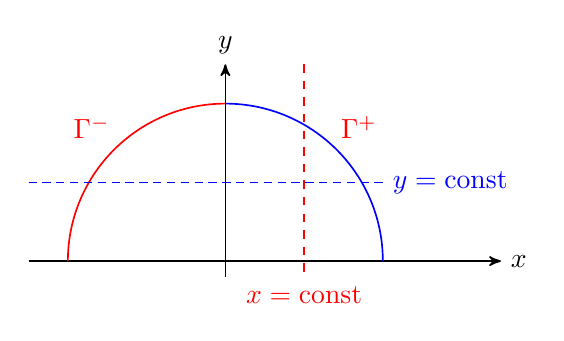
\begin{tikzpicture}[ media/.style={font={\footnotesize\sffamily}},
    interface/.style={
        postaction={draw,decorate,decoration={border,angle=-45,
                    amplitude=0.3cm,segment length=2mm}}},scale=2]

%\clip(-2,-2.4)rectangle(2.4,2.1);
\draw[semithick,->,>=stealth'](-1.25,0)--(1.75,0) node[right]{$x$};
\draw[semithick,->,>=stealth'](0,-0.1)--(0,1.25) node[above]{$y$};




\draw[semithick,red](-1,0) arc(180:90:1);
\node[red,semithick] at (135:1.2){$\Gamma^-$};
\draw[semithick,blue](1,0) arc(0:90:1);
\node[red,semithick] at (45:1.2){$\Gamma^+$};
\draw[blue,densely dashed,semithick] (-1.25,0.5)--(1,0.5) node[right]{$y=\textrm{const}$};

\draw[red,dashed,semithick] (0.5,1.25)--(0.5,-0.1) node[below]{$x=\textrm{const}$};


\end{tikzpicture}

\end{center}
\end{multicols}
\noindent 该解在与$x$轴平行的直线$y=\textrm{const}$上有相同的值, 因此不能满足$\Gamma^{+}$或$\Gamma^{-}$上的某一边界条件.
因此另一边界上出现边界层. 把原方程中的$y$看作参数, 并看作$x$为自变量的常微分方程, 由习题7.19知在$\Gamma^{+}$附近有边界层.
令
\[
\eta=\frac{x-x^{+}(y)}{\varepsilon}
\]
\[
u(x,y,\varepsilon)=V(\eta,y,\varepsilon)=V_{0}(\eta,y)+\cdots
\]
代入到原方程, 注意到
\[
\begin{array}{ll}
\displaystyle u_{x}=\frac{V_{\eta}}{\varepsilon}, & \displaystyle u_{xx}=\frac{V_{\eta\eta}}{\varepsilon^{2}}\\
\displaystyle u_{y}=V_{\eta}\frac{-{x'}^{+}(y)}{\varepsilon}+V_{y}, & \displaystyle u_{yy}=V_{\eta\eta}\Big[\frac{{x'}^{+}(y)}{\varepsilon}\Big]^{2}-V_{\eta}\frac{{x''}^{+}(y)}{\varepsilon}+2V_{y\eta}\frac{{x'}^{+}(y)}{\varepsilon}+V_{yy}
\end{array}
\]
可得
\begin{equation}
(1+[{x'}^{+}(y)]^{2})V_{\eta\eta}-V_{\eta}=0\label{eq:72901}
\end{equation}
其边界条件为
\[
V(0,y)=f^{+},V(-\infty,y)=f^{-}
\]
令$1+[{x'}^{+}(y)]^{2}=K$, 则方程(\ref{eq:72901})符合上述边界条件的解为
\[
V_{0}=(f^{+}-f^{-})e^{\eta/K}+f^{-}
\]


\vspace{1em}

\noindent 同样, 在与$y$轴平行的直线$x=\textrm{const}$上有相同的值, 因此不能满足$\Gamma$或$F$上的某一边界条件.
因此$F$上也出现边界层, 取内变量
\[
\xi=\frac{y}{\varepsilon^{\lambda}}, ~~ u(x,y,\varepsilon)=u(x,\xi,\varepsilon)=W(x,\xi)+\cdots
\]
代入到原方程, 注意到
\[
\begin{array}{ll}
\displaystyle u_{x}=W_{x}, & \displaystyle u_{xx}=W_{xx}\\
 &  \\
\displaystyle u_{y}=\frac{W_{\xi}}{\varepsilon^{\lambda}}, & \displaystyle u_{yy}=\frac{W_{\xi\xi}}{\varepsilon^{2\lambda}}
\end{array}
\]
可得
\[
\varepsilon\Big(\frac{W_{\xi\xi}}{\varepsilon^{2\lambda}}+W_{xx}\Big)=W_{x}
\]
为使$W_{\xi\xi}$与$W_{x}$同阶, $\lambda=1/2$. 因此上式变为
\[
W_{\xi\xi}-W_{x}=0
\]
其边界条件为
\[
W(x,0)=F(x), ~~ W(x,+\infty)=f(x), ~~ W(-R,0)=F(-R)=f(-R)
\]
符合上述边界条件$y=0$附近的内解为
\[
W_{0}=f(-R)+\int_{0}^{x+R}\frac{[F(\zeta)-f(-R)]\xi}{2\sqrt{\pi(x+R-\zeta)^{3}}}\exp\Big[\frac{-\xi^{2}}{4(x+R-\zeta)}\Big]d\zeta
\]

\end{solution}
